\documentclass{standalone}
\usepackage{tikz}
\begin{document}
    
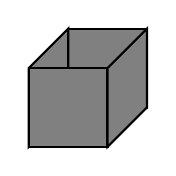
\begin{tikzpicture}[x=1cm,y=1cm,z=1cm,shift={(2,-1)}]
    \filldraw[black, thick, fill=gray!100] (0,0,0.5) -- (1,0,0.5) -- (1,1,0.5) -- (0,1,0.5) -- cycle;
    
    \filldraw[black, thick, fill=gray!100] (0,0,0) -- (0,0,0.5) -- (0,1,0.5) -- (0,1,0) -- cycle;
    \filldraw[black, thick, fill=gray!100] (0,0,0) -- (1,0,0) -- (1,1,0) -- (0,1,0) -- cycle;
   
     \filldraw[black, thick, fill=gray!100] (1,0,0) -- (1,0,0.5) -- (1,1,0.5) -- (1,1,0) -- cycle;
    %\filldraw[black, thick, fill=gray!100] (0,0,0) -- (0,1,0) -- (1,1,0) -- (1,0,0) -- cycle;
    %\filldraw[black, thick, fill=gray!100] (0,0,1) -- (0,1,1) -- (1,1,1) -- (1,0,1) -- cycle;
\end{tikzpicture}

\end{document}